\documentclass{beamer}

\usepackage[utf8]{inputenc}
\usepackage{epigraph}
\usepackage{tikz}

\usetikzlibrary{patterns, arrows, cd, positioning, backgrounds, fit, decorations.pathmorphing, shapes.misc, calc, matrix, decorations.pathreplacing, external}
\tikzset{%
  node/.style={draw, minimum size=12mm, inner sep=0mm, circle, fill=gray!50},
  edge/.style={thick},
  move/.style={->},
  brace/.style={
    decorate,
    decoration={brace,amplitude=10pt,mirror},
  },
  table nodes/.style={
    rectangle,
    draw=black,
    align=center,
    minimum height=7mm,
    text depth=0.5ex,
    text height=2ex,
    inner xsep=0pt,
    outer sep=0pt,
    inner sep=0pt
  },
  table/.style={
    matrix of nodes,
    row sep=-0.5pt,
    column sep=-0.5pt,
    nodes={
      table nodes
    }
  }
}


\usetheme{metropolis}
\metroset{numbering=fraction}

\title{A Grimm idea}
\subtitle{Exploring graphs with pebbles}
\author{Christoph Welzel}
\institute{Logik und Theorie diskreter Systeme, RWTH Aachen}

\begin{document}
\maketitle
\begin{frame}
  \frametitle{Motivation}
  \begin{itemize}
    \item Traversing Brobdingnagian graphs
    \item[$\rightarrow$] Web crawlers
    \item Agent moves over vertices along edges
    \item[$\Rightarrow$] Memory efficient agents
  \end{itemize}
\end{frame}

\begin{frame}
  \frametitle{Agents}
  \begin{quotation}
    Und als der volle Mond aufgestiegen war, so nahm Hänsel sein
    Schwesterchen an der Hand und ging den Kieselsteinen nach, die schimmerten
    wie neu geschlagene Batzen und zeigten ihnen den Weg.
  \end{quotation}
  \vspace{-0.5cm}
  \flushright{Brüder Grimm}
  \vspace{-0.5cm}
  \flushright{\emph{Hänsel und Gretel}}
  \begin{itemize}
    \item Agent carries set of markers $\rightarrow$ pebbles
    \item Leave pebbles on vertices
  \end{itemize}
\end{frame}

\begin{frame}
  \frametitle{Brobdignagian graphs}
  \begin{columns}
    \column{0.5\textwidth}
    \begin{itemize}
      \item Indistinguishable vertices
      \item Bounded degree ($\Delta$)
      \item Edges can locally enumerated $\left\{0,\dots,\Delta-1\right\}$ (Port)
      \item Agent is aware of:
        \begin{enumerate}
          \item Degree  of vertex
          \item Pebbles placed on vertex
          \item Pebbles carried by agent
          \item Port    agent entered vertex
        \end{enumerate}
    \end{itemize}
    \column{0.5\textwidth}
    \begin{center}
      \resizebox{\textwidth}{!}{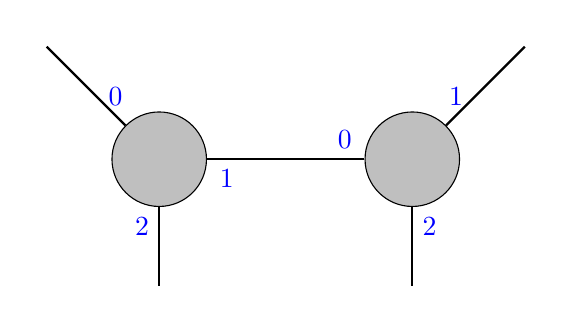
\begin{tikzpicture}
  \node[node] (m1) {};
  \node[node,right=2cm of m1] (m2) {};

  \node[above left=of m1] (e1) {};
  \node[below=of m1] (e2) {};

  \node[above right=of m2] (e3) {};
  \node[below=of m2] (e4) {};

  \draw[edge] (m1) to node[very near start, above] {\textcolor{blue}{0}} (e1);
  \draw[edge] (m1) to node[near start, left] {\textcolor{blue}{2}} (e2);

  \draw[edge] (m2) to node[very near start, above] {\textcolor{blue}{1}} (e3);
  \draw[edge] (m2) to node[near start, right] {\textcolor{blue}{2}} (e4);
  
  \draw[edge] (m1) to node[very near start, below] {\textcolor{blue}{1}} node[very near end, above] {\textcolor{blue}{0}} (m2);
\end{tikzpicture}
}
    \end{center}
  \end{columns}
\end{frame}

\begin{frame}
  \frametitle{Exploration sequence}
  \begin{columns}
    \column{0.5\textwidth}
    \begin{itemize}
      \item Describe movement of agent by relative turns
      \item $e_{1},\dots, e_{n}$
      \item For a vertex $v$ with degree $d_{v}$ which is entered on port $p$
        is left through port $p + e_{i}\mod p$
      \item<2->[$\rightarrow$] Example:
        $\only<3-3>{\colorbox{green}}{1}\;,\only<4-4>{\colorbox{green}}{3}\;,
        \only<5-5>{\colorbox{green}}{2}\;,\only<6-6>{\colorbox{green}}{2}$
    \end{itemize}
    \column{0.5\textwidth}
    \begin{center}
      \resizebox{\textwidth}{!}{\begin{tikzpicture}
  \node[minimum size=12mm,inner sep=0mm, circle] (8) {};
  \node[node,right=of 8] (6) {};
  \node[node,right=of 6] (7) {};
  \node[node,below=of 8] (0) {};
  \node[node,below=of 6] (1) {};
  \node[node,below=of 7] (2) {};
  \node[node,below=of 0] (3) {};
  \node[node,below=of 1] (4) {};
  \node[node,below=of 2] (5) {};
  \node[node,above right=0.5cm and 1cm of 2] (8) {};
  \node[node,below right=0.5cm and 1cm of 2] (9) {};

  \draw[edge] (0) to node[very near start, above] {0} node[very near end, above] {1} (1);
  \draw[edge] (1) to node[very near start, below] {0} node[very near end, above] {1} (2);
  \draw[edge,bend right] (2.north west) to node[very near start, right] {0} node[very near end, above] {2} (0);
  \draw[edge] (0) to node[very near start, right] {1} node[very near end, left ] {0} (3);
  \draw[edge] (3) to node[very near start, above] {1} node[very near end, below] {1} (4);
  \draw[edge] (4) to node[very near start, below] {0} node[very near end, below] {1} (5);
  \draw[edge] (5) to node[very near start, above] {0} node[very near end, below] {2} (1);
  \draw[edge] (1) to node[very near start, left ] {3} node[very near end, left ] {2} (6);
  \draw[edge] (6) to node[very near start, above] {0} node[very near end, above] {1} (7);
  \draw[edge] (8) to node[very near start, above] {0} node[very near end, right] {0} (7);
  \draw[edge] (8) to node[very near start, above] {1} node[very near end, right] {2} (5);
  \draw[edge] (9) to node[very near start, below] {1} node[very near end, below] {3} (5);
  \draw[edge,bend right=20] (9) to node[very near start, below] {0} node[very near end, below] {1} (6);

  \begin{scope}[on background layer]%
      \node [fit=(0)] (layer) {};%
  \end{scope}
  \begin{scope}[on background layer]%
      \node [fit=(4)] (layer) {};%
  \end{scope}
  \only<3-3>{\begin{scope}[on background layer]%
      \node [fit=(0), fill=green!50] (layer) {};%
  \end{scope}}
  \only<4-4>{\begin{scope}[on background layer]%
      \node [fit=(3), fill=green!50] (layer) {};%
  \end{scope}}
  \only<5-5>{\begin{scope}[on background layer]%
      \node [fit=(4), fill=green!50] (layer) {};%
  \end{scope}}
  \only<6-6>{\begin{scope}[on background layer]%
      \node [fit=(3), fill=green!50] (layer) {};%
  \end{scope}}
  \only<7-7>{\begin{scope}[on background layer]%
      \node [fit=(4), fill=green!50] (layer) {};%
  \end{scope}}


\end{tikzpicture}
}
    \end{center}
  \end{columns}
\end{frame}

\begin{frame}
  \frametitle{}
\end{frame}
\end{document}
